 \documentclass[book.tex]{subfiles}
\begin{document}
My personal introduction to computer gaming began in 1985, when my parents bought an MSX-1 home computer. I was fascinated by games such as Konami's \textit{Knightmare} and \textit{Nemesis 2}. It was not only the gameplay that intrigued me, but also how such games were created. This curiosity sparked my interest in programming and game development, and I soon began creating my first games in MSX-BASIC.\\

\par
Around the same time I was introduced to the MSX, Nintendo released \textit{Super Mario Bros.} for the Nintendo Entertainment System (NES). It became an instant blockbuster, combining colorful graphics with remarkably smooth side-scrolling. By comparison, the side-scrolling games I played on the MSX-1, such as Knightmare and Nemesis 2, moved at a constant, noticeably choppy speed.\\

\par
Super Mario Bros. was different. The player dictated the scrolling speed: you could accelerate from walking to running or jumping, and the screen would smoothly follow your actions. The game was immensely successful, both commercially and critically. It helped popularize the side-scrolling platform genre and served as a killer app for the NES\footnote{Upon release in Japan, 1.2 million copies were sold during its September 1985 release month. Within four months, about 3 million copies were sold in Japan.}. More importantly, it demonstrated the true power of the NES by utilizing a dedicated Picture Processing Unit (PPU) that handled sprites and scrolling independently of the CPU.\\


\par
My MSX-1 home computer lacked any hardware support for smooth scrolling. Other computers, like the MSX-2 and Commodore 64, could scroll up to 8 pixels (one character) horizontally or vertically. However, once that limit was reached, developers had to rely on all kinds of tricks to achieve continuous, full-screen smooth scrolling. This typically involved copying large amounts of data, simply to move the screen by a single character. Such approaches were extremely CPU-intensive and often beyond the capabilities of the hardware.\\

\trivia{Some great programmers succeeded in implementing smooth scrolling on the Commodore 64 and MSX-2, most notably in games such as \textit{Uridium} (1986) and \textit{Armalyte} (1988) on the Commodore 64, and \textit{Space Manbow} (1989) on the MSX-2.}\\


\par
The NES was one of the very first home consoles to offer true hardware-supported smooth scrolling. Essentially, the PPU had registers that could be written to, in order to set the fine (pixel) scroll. For example, to scroll the background 120 pixels horizontally and then 22 pixels vertically, you would first write the horizontal scroll value 120, followed by the vertical value 22 to the PPU\footnote{The PPU could only handle one-directional scrolling at a time. So bi-directional scrolling requires twice updating the PPU registers. }. Done deal! The video chip takes care of the rest, running at the same constant speed as it always has.\\

\begin{figure}[H]
  \centering
 \fbox{\includegraphics[width=1.0\textwidth]{screenshots_300dpi/Mario_Bros.png}}
\caption{Super Mario Bros on Nintendo Entertainment System}
\end{figure}

\par
In the late 1980s, the IBM PC lagged far behind the gaming power of the NES. It was designed for office work rather than gaming. It excelled at word processing and crunching numbers in spreadsheets. Although the PC game market was growing rapidly, it was dominated by adventure games (\textit{King's Quest}), role-playing games (\textit{Ultima series}), strategy titles, and simulations (\textit{SimCity}).
Action and platform games remained largely the domain of consoles and home computers, as the PC lacked hardware support for sprites and smooth scrolling.\\


\par
Then, on December 14\textsuperscript{th}, 1990, a small, unknown software company called "Ideas from the Deep" released \textit{Commander Keen in Invasion of the Vorticons} for the PC. It was the first PC game to feature smooth side-scrolling, similar to Super Mario Bros on the NES. \\

\begin{figure}[H]
  \centering
 \fbox{\includegraphics[width=1.0\textwidth]{screenshots_300dpi/Keen_Verticons.png}}
\caption{Commander Keen in Invasion of the Vorticons}
\end{figure}

\par
So how was it possible to create a game like Commander Keen on the IBM PC?\\



\par
With the introduction of the IBM AT, powered by the Intel 80286, the PC began to outperform consoles and home computers on the market. In terms of raw processing power, not even the NES could compete with the IBM AT.\\



\par
But raw power was about the only area in which the PC excelled. Its other components were notoriously difficult to master:
\begin{itemize}
  \item The video adapter (called EGA) did not support hardware scrolling. It also lacked hardware sprites, which would have allowed objects to move on the screen simply by updating their \cw{(x,y)} coordinates.
  \item The PC speaker could produce little more than a series of (mostly) annoying "beeps". Sound cards did exist, but they were still in their infancy and far from standardized.
  \item Memory available to applications was 640KiB, much more than an average home computer, which typically had 64KiB. However, RAM was not organized as a flat address space but accessed through segments and offsets. Different memory models existed, each involving trade-offs between program size and performance.
\end{itemize}


\par
\begin{figure}[H]
\centering
  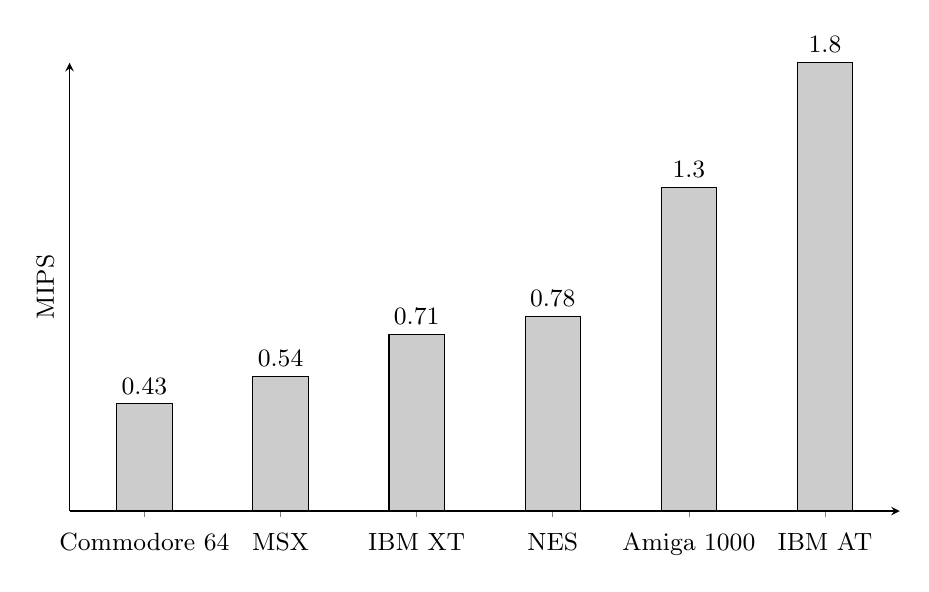
\begin{tikzpicture}[font=\small]
    \begin{axis}[
      width=\textwidth,
      height=0.6\textwidth,
      ybar=6pt,
      bar width=20pt,
      ylabel={MIPS},
      ymin=0,
      ytick=\empty,
      xtick=data,
      axis x line=bottom,
      axis y line=left,
      enlarge x limits=0.11,
      symbolic x coords={Commodore 64, MSX, IBM XT, NES, Amiga 1000, IBM AT},
      xticklabel style={anchor=base,yshift=-\baselineskip},
      nodes near coords={\pgfmathprintnumber\pgfplotspointmeta}
    ]
      \addplot[fill=black!20,draw=black] coordinates {
        (Commodore 64, 0.43)
        (MSX, 0.54)
        (IBM XT, 0.71)
        (NES, 0.78)
        (Amiga 1000,1.3)
        (IBM AT, 1.8)
      };
    \end{axis}
   \end{tikzpicture}
   \caption{Consoles\protect\footnotemark and IBM PC CPU comparison (MIPS)\protect\footnotemark $^,$\protect\footnotemark.}
   \label{fig:ems_xms_layout}
 \end{figure}
 \addtocounter{footnote}{-2}
 \footnotetext{The Commodore 64 uses a MOS 6510 CPU running at 1MHz. The MSX uses a Zilog Z80 running at 3.6MHz. The Amiga 1000 has a Motorola 68000 CPU  running at 7.16 MHz. The NES uses a Ricoh 2A03 CPU running at 1.8 MHz.}
 \stepcounter{footnote}
 \footnotetext{Million Instructions Per Second.}
 \stepcounter{footnote}
 \footnotetext{Gamicus Fandom: https://gamicus.fandom.com/wiki/Instructions\_per\_second.}


\par
Overall, creating a fast side-scrolling action game on the PC seemed nearly impossible. Nevertheless, programmers around the world embraced the challenge, exploring the depths of the hardware and produced remarkable games. Their ingenuity is what inspired me to write this book.\\

\par
This book is divided into three chapters:
\begin{itemize}
  \item Chapter 2: The Hardware. An exploration of the main PC components from 1990 and the challenges they presented.
  \item Chapter 3: The tools and assets. Which tools are used for game development and how assets are created and structured.
  \item Chapter 4: The Software. A deep dive into the Commander Keen game engine and how the team bent the hardware to their will. Commander Keen targeted the 16-color EGA graphics card, but a CGA version was also released, which is discussed in this chapter as well.

\end{itemize}


\par
This book focuses on \textit{Commander Keen in Keen Dreams}, which was developed after the first three releases in the series. The reason for this choice is straightforward: it is the only version with publicly released source code. Where relevant, I will also highlight technological differences across the versions of Commander Keen. However, code examples will be limited to Keen Dreams due to the availability of the source material.\\

\begin{figure}[H]
  \centering
 \fbox{\includegraphics[width=1.0\textwidth]{screenshots_300dpi/Keen_Dreams.png}}
\caption{Commander Keen in Keen Dreams}
\end{figure}








\end{document}